%%%%%%%%%%%%%%%%%%%%%%%%%%%%%%%%%%%%%%%%%%%%%%%%%%%%%%%%%%%%%%%%%%%%%%
\clearpage
\section{Calling an Application}
\label{sec:calleval}

Every optimization application must provide a way for HOPSPACK to compute the
objective function and nonlinear constraint values at a given point.
HOPSPACK provides a simple and flexible method using system calls, described
in \SECREF{subcalleval:systemcall}.
The user can also modify HOPSPACK source code to evaluate points in some
other manner, as discussed in \SECREF{subcalleval:inlineeval}.


%%%%%%%%%%%%%%%%%%%%
\subsection{Evaluation by System Call}
\label{subcalleval:systemcall}

The default mechanism in HOPSPACK is to call an external program for
function evaluations.  Generally, the user writes
a simple wrapper that calls the true application.
Variable values are passed in a short text file and function
results are passed back in a separate text file.  HOPSPACK writes the variable
values, makes a system call from C++ to execute the application,
waits for it to complete, and reads the output file.
This simple mechanism provides maximum flexibility for the application.
It can be written in any language (Fortran, C, C++, Perl, MATLAB, etc.),
consist of multiple executables strung together (e.g., using
a shell or .bat script),
and reference external data sources.
The application itself can use MPI to run in parallel, although HOPSPACK
will not adjust its load balancing (you must figure how to allocate nodes
between HOPSPACK and the application copies).
The same application wrapper will work with the MPI, multithreaded, and serial
versions of HOPSPACK.

\begin{figure}[!h]
  \begin{center}
    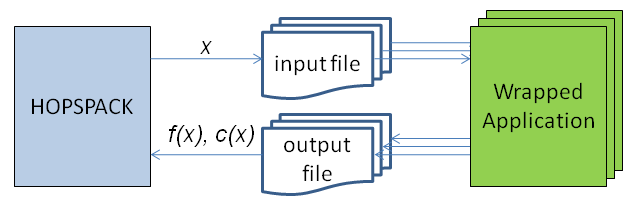
\includegraphics[width=4.0in]{EvalDiagramClipped.png}
    \vspace{-5mm}
  \caption{HOPSPACK communication with an application.}
  \label{fig:callforeval}
  \end{center}
\end{figure}

Figure~\ref{fig:callforeval} shows the flow of data from HOPSPACK to an
application.  Specific variable values at a trial point $x$ are written
to an input file, and the evaluated objective $f(x)$ plus any
nonlinear constraints $c(x)$ are returned via an output file.
%
The figure shows multiple instances of the application running in parallel.
Each instance has its own input and output files, and must run independent
from other application instances.
Figures~\ref{fig:evalMPI} (MPI) and \ref{fig:evalMT} (MT) show examples of how
the applications and HOPSPACK might be distributed across processors and threads.
HOPSPACK helps maintain independence of parallel application instances
by defining a unique ``tag number'' for each evaluation point.  The tag is
used to form unique input and output file names and is made available to
the application instance.  Input and output file names are generated by
HOPSPACK as the concatenation of a string
defined by parameter {\tt Input Prefix} (\PGREF{param:EV-inprefix})
or {\tt Output Prefix} (\PGREF{param:EV-outprefix}), the tag number, and
the evaluation type (discussed below).
The unique tag number allows all files to coexist in the same directory.
If the application creates temporary files, it should use the tag number
to name the files so there is no conflict between parallel instances.
Tag numbers are generated from a counter that is reset whenever HOPSPACK starts;
hence, tag numbers can be reused when HOPSPACK restarts.
 
Input and output file information depends on the type of evaluation information
desired, which is one of the following:
\vspace{-11pt}
\begin{tabbing}
  xxxxxxxxxx \= xxxxx \= \kill
  \> {\tt F}  \> Evaluate the objective $f(x)$ only (no constraints)  \\
  \> {\tt C}  \> Evaluate nonlinear constraints $c(x)$ only (no objective)  \\
  \> {\tt FC} \> Evaluate $f(x)$ and nonlinear constraints $c(x)$
\end{tabbing}
The default type is {\tt FC} since the GSS solver requires all information
at each trial point.  However, a different solver might separate processing
of the objective and constraints; for example, a solver may want to first
find a completely feasible point before requesting the objective value.

The input file begins with two lines of header information and then the value
of each variable.  The first line contains the evaluation type,
and the second line gives the number of variables.
This is followed by variable values, one per line.
The text below shows an example of an input file generated by HOPSPACK for
a problem with two variables:
\vspace{-11pt}
\begin{verbatim}
    FC
    2
    -1.50000000000000e+00
    3.91875000000000e+00
\end{verbatim}

The output file format is similar, with the objective and constraint values
written as vectors in one file.
Objective values are written first
(assuming the evaluation type is {\tt F} or {\tt FC}), and then any nonlinear
constraints (for type {\tt C} or {\tt FC}).
Objective values are written as a vector to allow applications
with multiple objectives.  Constraints are written as
two vectors of values:  one for equalities and one for inequalities.
In all three cases the format of a vector begins with a header line giving
the number of items, and then a list of values, one per line.
If a function cannot be evaluated, the string ``{\tt DNE}'' should be returned,
indicating a value does not exist at the trial point.
The text below shows an example of an output file for type {\tt FC}.
There is one objective (with $f(x) = 5$), no equality constraints,
and two inequalities.
Nonlinear inequalities follow a ``greater than zero'' convention
(\SECREF{subconfig:DEFINITION}), so this particular point is feasible
with respect to the first inequality and infeasible with respect to the second.
Note that HOPSPACK expects the number of objectives to match the value
of configuration parameter
{\tt Number Objectives} (\PGREF{param:PD-numobjs}), and the number of
constraints to match {\tt Number Nonlinear Eqs} (\PGREF{param:PD-numeqs})
and {\tt Number Nonlinear Ineqs} (\PGREF{param:PD-numineqs}).
\vspace{-11pt}
\begin{verbatim}
    1
    5.00000000000000e+00
    0
    2
    1.25000000000000e+02
    -2.08164062500000e+00
\end{verbatim}

When the application wrapper is called to evaluate a particular trial point,
it is given four command line arguments:  the input file name, output file name,
tag number, and evaluation type.  The last argument is repeated on the
first line of the input file.
The application wrapper must read a HOPSPACK input file and create a new
output file before completing.  The wrapper executable itself should return
zero if successful; any other value indicates to HOPSPACK that the evaluation
failed.
An example written in C is provided in the file
{\sf examples/1-var-bnds-only/var\_bnds\_only.c}.  Examples written in C++
are provided in similar subdirectories, including a problem with nonlinear
constraints in {\sf examples/4-nonlinear-constraints/nonlinear\_constraints.cpp}.
The HOPSPACK source code that calls the application is located in
{\sf src/src-evaluator/HOPSPACK\_SystemCall.cpp}.

The application wrapper can return a short error message that will be
reported in HOPSPACK output and passed to solvers.  The point will be
marked as unevaluated, causing it to be ignored by most solvers.
The error message can be a useful mechanism for reporting types of evaluation
failures, instead of simply failing.
If the {\tt Display} parameter from the ``Mediator'' sublist is set to 3
or higher, then the Mediator will print a summary list at the end of execution
showing all evaluation messages that were received.
To send an error message the wrapper executable should return zero
(as though it succeeded), and the message should be on the first line of
the output file instead of the number of objectives.  Everything after the
message will be ignored.
HOPSPACK will attach the message to the point and notify all solvers that
the point could not be evaluated.


%%%%%%%%%%%%%%%%%%%%
\subsection{Linking Evaluation Code}
\label{subcalleval:inlineeval}

The default HOPSPACK mechanism described in \SECREF{subcalleval:systemcall}
evaluates functions by calling the application as a separate process.
A user familiar with C++ can instead link HOPSPACK with the application
code and call it directly.  This mechanism eliminates separate application
processes and file-based communications.  Direct calls will therefore run faster,
although the time savings may be negligible compared to function evaluation
times.
Direct calls also allow run time control of the application through
customization of the ``Evaluator'' sublist of configuration parameters.

Calling the application directly requires modification of HOPSPACK source
code, and linking generally requires changing a CMake build file.
An example is provided in the directory {\sf examples/linked-evaluator-example}.
This example contains a custom {\tt ExampleLinkedEvaluator} class
that implements the {\tt HOPSPACK::Evaluator} interface.  The new class
includes methods {\tt evalF()} and {\tt evalFC()} for computing the
objective function and nonlinear constraints of a specific application.
The example shows how to modify the {\tt HOPSPACK::EvaluatorFactory} class
so it supplies instances of {\tt ExampleLinkedEvaluator}.
More information is given in the file
{\sf examples/linked-evaluator-example/README\_linked\_evaluator.txt}.

If the application depends on specific libraries, then their names must be
given to CMake.  See \SECREF{subsec:cmakeaddlib} for details.

An application called directly has the potential to crash HOPSPACK.
Be sure to surround the call with {\tt try/catch} handlers to trap any
application errors.  If an error is found, the custom evaluator should
return {\tt DNE} values for the functions and a short error message that
will be reported in HOPSPACK output.

An application called directly from the multithreaded version of HOPSPACK must
be thread safe.  HOPSPACK may call {\tt evalFC()} simultaneously
from many threads in the same shared memory space.
%TBD mention AMPL ASL?


%%%%%%%%%%%%%%%%%%%%
\subsection{Evaluation Tips}

For best results, applications should use full numerical precision when
passing values.  HOPSPACK writes variable values to the input file
with 15 significant digits, the maximum number of meaningful digits for double
precision on most machines.  The number of digits can be modified with the
configuration parameter {\tt File Precision} (\PGREF{param:EV-prec}).
The application wrapper should write results to the output file using the
most precision possible.

An application with nonlinear constraints might benefit from careful ordering
of calculations in the application wrapper.  For instance, if some constraints
cannot be violated (sometimes called ``hard constraints''), then it may be
best to check this first and not try to compute the objective function at
an infeasible point.
In this case it is appropriate to return {\tt DNE} for any unevaluated functions.
If the objective is well defined but expensive to compute, then it may be
best to skip evaluating at an infeasible point, returning {\tt DNE} for the
objective.  This causes the constraint to appear as an infinite barrier to
solvers, because an objective value of {\tt DNE} is treated as a value of
infinity ($+\infty$ if minimizing, $-\infty$ if maximizing).
An infinite barrier is nonsmooth and could slow convergence, but the overall
time savings might be worthwhile.

Some solvers might not be capable of working with nonlinear constraints.
In this case the evaluation might choose to return {\tt DNE} when a point
is infeasible.  However, this is not recommended if using the default GSS
solver in HOPSPACK.  GSS computes a penalty for infeasible points and can
make use of the extent to which a point violates constraints.
See \SECREF{subgss} for more.
